\chapter{mainloop} 
\label{sec:listing}
\lstset{style=68KStyle}
\lhead[tempest 2000]{}

Unlike Tempest, the engine that runs Tempest 2000 is not contained within a mainline routine. Instead
the donkey work is done during a vertical sync interrupt. Vertical sync is a point in time: specifically
when the Atari Jaguar has finished writing pixels to the screen and has a short amount of time available
before it starts writing pixels again from the top. An interrupt is a routine the system will call at a moment
of the programmer's choosing. A vertical sync interrupt is when you combine the two, and in this case they 
are combined in a routine called \icode{Frame}. It is this routine that manages the state of the game and prepares
all the objects for display and the sound for output.

That said, Tempest 2000 does have a mainline routine but it is there to solve a problem encountered in development
rather than as part of a grand design. As we shall see there are a number of ways of generating graphical data on the Atari
Jaguar, and two of them have their own dedicated processors. These are the Graphics Processor (GPU), which specializes
in the fast trigonometric operations required for 3D displays and the Blitter, which is suited for large copy and fill operations.
It is worth being clear that neither of these processors or any of their operations actually write graphics to the screen.
Instead this function is performed by a third dedicated processing unit, the Object Processor. It is the Object Processor 
that turns data into light. This unit takes a list of operations set up by the programmer for each frame and uses them to write
pixels to the screen. These operations will usually include data prepared by the GPU and the Blitter in a long list of tasks
for the Object Processor known as an Object List. It's the programmer's job to have a new Object List ready every time
the Object Processor is about to paint the screen. 

It was the initial intention that the \icode{Frame} routine would be solely responsible for this task in Tempest 2000. 
But there was a snag: it kept crashing. We know this because Jeff Minter left us one of his rare comments at the head
of the \icode{mainloop routine}:

\begin{lstlisting}[escapechar=\%]
; This loop runs the GPU/Blitter code.  I found that if you
; started up the GPU/Blitter pair from inside the FRAME
; Interrupt, the system would fall over if they got really heavily
; loaded.  MAINLOOP just waits for a sync from the FRAME routine,
; launches the GPU, then loops waiting for another sync.

mainloop:
      move #1,sync      ; Reset the sync.
      move #1,screen_ready ; Signal to 'Frame' screen ready for display.
      move pauen,_pauen ; Reset the pause indicator.
  
main: tst sync          ; Loop waiting for another sync..
      bne main          ; from the interrupt in 'Frame'.
  
      move #1,sync      ; Reset sync so that we wait for a new frame.
      ; Use dscreen as the screen that GPU will draw everything to.
      move.l dscreen,gpu_screen  
  
      ; Do the actual mainloop work, mainloop_routine is usually 
      ; a reference to the 'draw_objects' routine.
      move.l mainloop_routine,a0 ; Move mainloop_routine to a0. 
      jsr (a0)          ; Call mainloop_routine. 
\end{lstlisting}

So instead of doing all the necessary GPU and Blitter operations during a vertical sync interrupt, we do them
here in this \icode{mainloop}. Notice the busyloop in the second paragraph above where we wait for the value in \icode{sync}
to change to a zero. This forces the CPU to wait until the \icode{Frame} routine resets it to zero. Once it has
been reset we can go ahead and execute our \icode{mainloop\_routine}. This is actually a reference to the 
\icode{draw\_objects} routine - and it is this routine that does all the GPU and Blitter work required to calculate
the pixels for display.

Here we see that when the game is initialized, \icode{draw\_objects} is selected as the destination for
\icode{mainloop\_routine}, and then we enter the \icode{mainloop}.
\begin{lstlisting}
        ; The common entry point for single-player and head-to-head games.
go_in:  move.l #rotate_web,routine
        move.l #0,warp_count
        move.l #draw_objects,mainloop_routine
        move pauen,_pauen
        clr db_on             ; Enable double-buffering.
        bra mainloop          ; Enter the mainloop until we lose a life.
\end{lstlisting}

We will investigate the mechanics of using the GPU and the Blitter in later sections, but for now let's get a
sense of the kind of things the \icode{draw\_objects} routine uses the GPU and Blitter for.
A quick glance through the top of the routine shows us drawing the starfield (\icode{dostarf}).

\section*{drawing objects}
\begin{lstlisting}[escapechar=\%]
draw_objects:
        bsr clearscreen            ; Clear the screen.
        move.b sysflags,d0         ; Copy sysflags to d0.
        and.l #$ff,d0              ; Keep it between 0 and 255.
        move.l d0,_sysflags        ; pass sys flags to GPU
        tst sf_on                  ; Is the starfield active?
        bne dostarf                ; If yes, go to 'dostarf'.
        bra gwb                    ; Otherwise do the web.
    
        ; Prepare the starfield!
dostarf:
        move.l #3,gpu_mode         ; mode 3 is starfield1 in llama.gas
        move.l vp_x,in_buf+4       ; Put x pos in the in_buf buffer.
        move.l vp_y,in_buf+8       ; Put y pos in the buffer.
        move.l vp_z,d0             ; Get the current z pos.
        add.l vp_sf,d0             ; Increment it.
        move.l d0,in_buf+12        ; Add it to the buffer.
        move.l #field1,d0          ; Get the starfield data structure.
        move.l d0,in_buf+16        ; And put it in the buffer.
        move.l warp_count,in_buf+20   ; Add the warp count.
        move.l warp_add,in_buf+24   ; Add the warp increment.
        lea fastvector,a0          ; Get GPU routine to use in llama.gas.
        jsr gpurun                 ; do gpu routine
        jsr gpuwait                ; Wait until its finished.
\end{lstlisting}

As you can see 'doing the starfield' involves setting up a number of registers and variables
before finally invoking the GPU (\icode{jsr gpurun}) to do its magic and waiting for it to finish
(\icode{jsr gpuwait}). We will take a closer look at the mechanics of starfield generation in a later
chapter, but the above begins to give us a flavour of the formula required to get a GPU routine up 
and running.

The next element we find is a routine for drawing the playfield of Tempest 2000: the web. As you can
see there is a lot going on here and the truth is, this isn't even all of it. And not just that,
there are a number of different GPU routines used for drawing webs scattered throughout the game depending
on the mode we are playing or whether there is more than one player. Just looking briefly through the code
below (and you should confine yourself to that for now) gives you a sense of the overhead involved in setting
up a reasonably complex piece of GPU code. Note that at the end of the listing below we load a variable called
\icode{equine2} to the \icode{A0} register. This is an address to the actual GPU code that the Graphics Processor
will run, using all the data set up in the previous lines. So there is much more complexity and detail underneath,
even here. We will cover this in more detail in the chapter devoted to webs.

\begin{figure}[H]
      \centering
      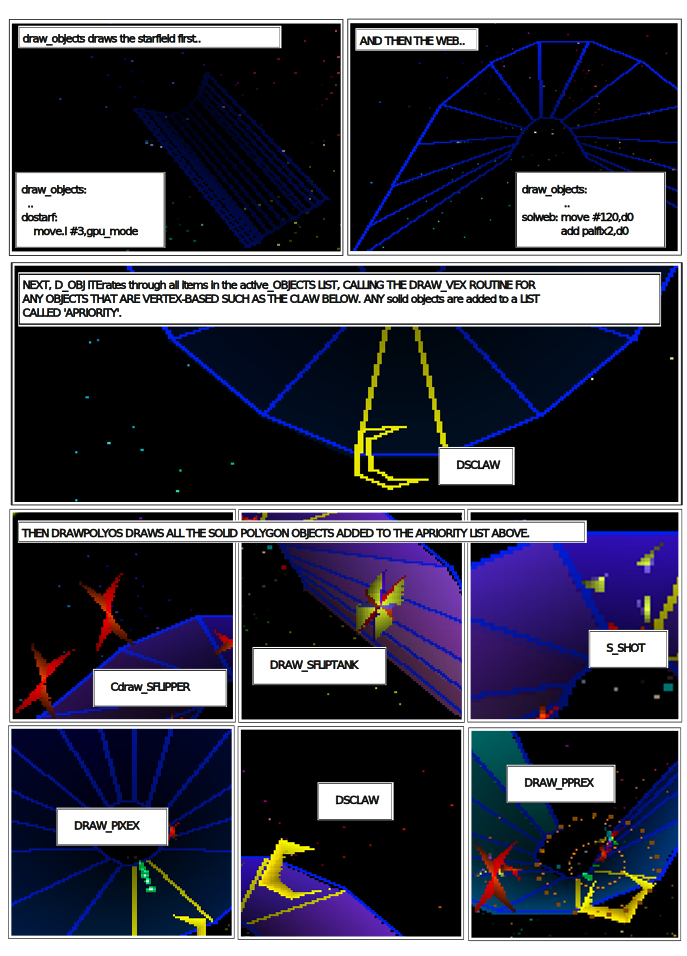
\includegraphics[width=13.7cm]{src/mainloop/mainloop-draw_objects-comic.png}%
\end{figure}

\begin{lstlisting}[escapechar=\%]
gwb:    move.l vp_x,d3
        move.l vp_y,d4
        move.l vp_z,d5
    
solweb: move #120,d0
        add palfix2,d0             ; Adjust for PAL screens if required.
        and.l #$ff,d0              ; Keep it between 0 and 255
        move.l d0,ycent
        tst l_solidweb
        beq vweb
        cmp #1,webcol              ; our 'transparent' webs...
        beq vweb
        lea _web,a6                ; draw a solid poly Web
        tst 34(a6)
        beq n_wb
        lea in_buf,a0              ; Point our GPU RAM input buffer at a0.
        move.l 46(a6),d0
        move.l d0,(a0)
        move.l 4(a6),d0            ; Get the source X position.
        sub.l d3,d0
        move.l d0,4(a0)
        move.l 8(a6),d0            ; Get the object's Y position.
        sub.l d4,d0
        move.l d0,8(a0)
        move.l 12(a6),d0           ; Get the object's Z position.
        sub.l d5,d0
        bmi n_wb
        move.l d0,12(a0)
        move l_solidweb,d0
        and.l #$ff,d0              ; Keep it between 0 and 255
        move.l d0,16(a0)
        move 28(a6),d0
        and.l #$ff,d0              ; Keep it between 0 and 255
        move.l d0,24(a0)
        move frames,d0             ; Stash the frame count in d0.
        and.l #$ff,d0              ; Keep it between 0 and 255
        move.l d0,28(a0)
        move.l #w16col,32(a0)
        move.l #0,gpu_mode         ; Select the web3d shader in donky.gas.
        lea equine2,a0             ; Load the GPU module in donky.gas.
        jsr gpurun                 ; Run the selected GPU module.
        jsr gpuwait                ; Wait for the GPU to finish.
        jsr WaitBlit               ; Wait for the blitter to finish.
\end{lstlisting}
You may note at the end that we call a routine called \icode{WaitBlit}. This is because in addition to computing the
polygons that make up the 3D web, the GPU also 'blits' or writes its results to a buffer that will ultimately be used
by the Object Processor to write the pixels to the screen. It is this dual operation that caused Minter a headache
when attempting it from within the vertical sync interrupt. (My own suspicion is that there just wasn't enough time in the
interrupt to do everything he wanted on the GPU and Blitter - so moving it here to the mainloop ensured that it would only
be done opportunistically and at the risk of missing a frame every now and then.)

But there is more to Tempest 2000 than starfields and webs so there must be plenty of other things being drawn in here too.
At first it is not easy to see where though. The next section of the \icode{draw\_objects} routine is cryptic at best 
but on close inspection does contain some clues. As elsewhere, I've added comments to assist understanding:

\begin{lstlisting}
n_wb:   move.l activeobjects,a6 ; activeobjects is a list of things to draw!
        bsr d_obj
        bra odend

        ; A loop for processing everything in 'activeobjects'.
d_obj:  cmpa.l #-1,a6         ; Have we reached the end of activeobjects?
        beq oooend            ; If yes, skip to end.
        move 50(a6),d0        ; Is the object marked for deletion?
        beq no_unlink         ; If not, skip to no_unlink and draw it.
    
        ; This verbose section up until no_unlink is concerned entirely
        ; with deleting the dead object from the activeobjects list.
        move.l 56(a6),d1      ; Get address of previous object.
        bmi tlink             ; 
        move.l d1,a5          ; Move previous object to a5.
        move.l 60(a6),60(a5)  ; Make it invisible to the vsync interrupt.
    
tlink:  move #-1,50(a6)       ; mark it bad
        move.l 60(a6),-(a7)   ; Stash the next object address
        move d0,-(a7)         ; Stash some values in the stack so we can restore them later.
        move.l a6,a0
        move 32(a6),-(a7)     ; save player ownership tag
        move (a7)+,d1         ; Restore stashed values from the stack.
        move (a7)+,d0         ; Restore stashed values from the stack.
        lea uls,a1            ; Point a1 at uls.
        asl #2,d0             ; Multiply it by 4.
        move.l -4(a1,d0.w),a1 ; Use d0 as an index in to 'uls'.
        jmp (a1)              ; Jump to the entrypoint below selected by the index.
    
        ; Object specific unlinking/deletion routines
uls:    dc.l afinc,ashinc,pshinc
    
pshinc: tst d1                ; player ownership of an unlinked bullet
        beq ulsh1
        add #1,shots+2
ulo:    move #1,locked        ; Lock the activeobjects list while we delete from it.
        bsr unlinkobject      ; Remove the object from the active objects list.
        clr locked            ; Unlock the activeobjdects list again.
        bra nxt_o             ; Finished deleting, go the the next object.
ulsh1:  add #1,shots
        bra ulo
    
ashinc: add #1,ashots
    
afinc:  add #1,afree          ; Make the slot available for a new activobject.
        bra ulo
    
        ; Actually draw the object.
        ; No need to remove the object, just draw it.
no_unlink:
        lea draw_vex,a0       ; Get our table of draw routines.
        move 34(a6),d0        ; Is this object smaller than a pixel?
        bpl notpxl            ; If not, go to notpxl.
        move.l #draw_pel,a0   ; Use draw_pex for pixel-size objects.
        bra apal              ; Jump to the draw call.
notpxl: asl #2,d0             ; Multiply the val in d0 by 4.
        move.l 0(a0,d0.w),a0  ; Use it as an index into draw_vex.
apal:   move.l 60(a6),-(a7)   ; Store the index of next object in a7.
        jsr (a0)              ; But first call the routine in draw_vex.
        jsr gpuwait           ; Wait for the GPU to finish.
nxt_o:  clr locked            ; Clear 'locked' just in case.
nxt_ob: move.l (a7)+,a6       ; Put the index of next object back in a6.
        bra d_obj             ; Go to the next object.
oooend: rts

\end{lstlisting}

This part of the \icode{draw\_objects} routine is concerned with processing a linked list called
\icode{activeobjects} using a loop that runs from \icode{d\_obj} to \icode{bra d\_obj} in the second
last line from the end. This \icode{activeobjects} list contains the detail for all objects that
are active on the screen and require drawing by the GPU/Blitter. Some of the original (but sparse)
code comments added by Minter suggest that this was initially conceived as a list for managing just
the player and enemy bullets but it expanded over time. 

Each object in the \icode{activeobjects} list has the following structure:

\begin{figure}[H]
  {
    \setlength{\tabcolsep}{3.0pt}
    \setlength\cmidrulewidth{\heavyrulewidth} % Make cmidrule = 
    \begin{adjustbox}{width=9cm,center}

      \begin{tabular}{lll}
        \toprule
        Bytes & \\
        \midrule
        0-4 & Vector Object or Solid Object \\ 
        4-8 &  X \\
        8-12 &  Y \\
        12-16 &  Z \\
        16-20 & Position on web.\\
        20-24 & Velocity \\
        24-28 & Acceleration  \& XY orientation \\
        28-30 & XZ Orientation \& XZ orientation  \\
        30-32 & Y Rotation \\
        32-34 & Z Rotation \\
        34-36 & Index into draw routine in \icode{draw\_vex}.\\
        36-38 & Start address of pixel data. \& Delta Z \\
        38-40 & Y & Colour change value\\
        40-42 & Colour \\
        42-44 & Scale factor \\
        44-46 & Mode to climb, descend or cross rail \\
        46-48 & Size of Pixel Data  \& Duration.\\
        48-50 & Fire Timer \\
        50-52 & Marked for deletion \\
        52-54 & Whether an enemy or not. \\
        54-56 & Object Type \\
        56-60 & Address of Previous Object \\
        60-64 & Address of Next Object \\
        \bottomrule
      \end{tabular}
    \end{adjustbox}
  }\caption*{The structure of objects in \icode{activeobjects}.}
\end{figure}

So in the 64 bytes of each object we cover quite a bit of ground. There is colour, co-ordinate, motion, and orientation
information. There's also detail that defines the behaviour of the object and most immediately relevant to what
we are looking at here, an index into the draw routine to use for the object at bytes 34-36.

This index is a value that references the routine given at the appropriate position in the \icode{draw\_vex} array:
\begin{lstlisting}
draw_vex: 
         dc.l rrts,draw,draw_z,draw_vxc,draw_spike,draw_pixex,draw_mpixex,draw_oneup,draw_pel,changex
         dc.l draw_pring,draw_prex,dxshot,drawsphere,draw_fw,dmpix,dsclaw,dsclaw2
\end{lstlisting}

The draw routine can vary depending on the type of object. There's a distinct treatment of vector object and objects
that are solid polygons. Vector objects require the least work and if the header in bytes 0-4 indicates that it requires
vector drawing only (for example the player's claw) then a vector draw in the GPU will suffice. The \icode{draw} routine
in the second item in \icode{draw\_vex} is the base routine for deciding whether a vector draw is sufficient or not, and
most of the other routines make use of it in addition to the object-specific detail they manage:

\begin{lstlisting}
draw:
        move.l a6,oopss   ; Stash the header.
        move.l (a6),d0    ; Is the header value greater than zero?
        bpl vector        ; If yes, then a vector draw will suffice.

        ; Otherwise we need to do add this object to the 'apriority'
        ; list so that it can be drawn as a solid polygon.

        ; The 'apriority' list stores objects in the descending order
        ; of their Z co-ordinate. This ensures that nearer objects are
        ; painted in front of objects that are further away or 'behind' them.
        move.l fpriority,a0  ;get a free priority object
        move.l a6,(a0)
        move.l 12(a6),d0  ;get 'z'
        move.l d0,12(a0)  ;put z in prior object
        move.l apriority,a1
        move.l a1,a2
chklp:
        cmp.l #-1,a1       ;no objects active?
        bne prio1
        bra insertprior    ;we are at top of list then, if we are first a1=a2=-1

prio1:
        cmp.l 12(a1),d0    ;check against stored 'z'
        bge insertprior    ;behind, insert on to list
        move.l a1,a2
        move.l 8(a1),a1    ;get next object
        bra chklp    ;loop until list end or next object in front of us
        rts      ;return with object at right place in the list
\end{lstlisting}

Reading through the above we can see that if a \icode{vector} draw won't do the job then the object gets
added to a list called \icode{apriority} and nothing else is done with it for now. So what we are doing in our
\icode{d\_obj} loop is a first pass through the \icode{activeobjects} list, with any items on the list that 
require attention to the order in which they are painted, passed off to the \icode{apriority} list. Notice
that we don't mutate or update the objects in any way, we simply pass them over so the structure of the objects
we described above remains unchanged.

Once we have finished this first run through the \icode{activeobjects} list our next order of business
is to process the \icode{apriority} list we've populated. This is done in \icode{drawpolyos} which we
call right after we've finished with our first pass of \icode{activeobjects}. 

\begin{lstlisting}
        ; We've finished our first pass of activeobjects.
odend:
        bsr showscore     ; Show the score.
        ; In Tempest Classic mode we don't need solid polygons.
        tst blanka        ; Are we doing solid polygons?
        beq odvec         ; If not, skip.
        bsr drawpolyos    ; if we are, draw them.
\end{lstlisting}

Drawing our polygons happens below. We iterate through the 'apriority' list, deleting items in it
as we go, and calling the object-specific draw routine for each to render them to the screen.

\begin{lstlisting}
solids: 
        dc.l rrts,cdraw_sflipper,draw_sfliptank,s_shot,draw_sfuseball
        dc.l draw_spulsar,draw_sfusetank,ringbull,draw_spulstank
        dc.l draw_pixex,draw_pup1,draw_gate,draw_h2hclaw,draw_mirr
        dc.l draw_h2hshot,draw_h2hgen,dxshot,draw_pprex,draw_h2hball
        dc.l draw_blueflip,ringbull,supf1,supf2,draw_beast,dr_beast3
        dc.l dr_beast2,draw_adroid            

; Routine for drawing all solid polygons.
; Process each object in the 'apriority' list. We remove each item after
; processing.The draw routine for each item is given by its index into
; the 'solids' array.
drawpolyos:
        move.l #192,xcent   ; Set 192 as X centre.
        move.l #120,d6      ; Set 120 as Y centre.
        add palfix2,d6      ; Adjust for PAL if necessary.
        move.l d6,ycent     ; Store it as Y centre.
        move.l apriority,a0 ; Get our 'apriority' list.
dpoloop:
        cmp.l #-1,a0
        beq rrts            ; End of list was reached
        move.l (a0),a6      ; Get the index to 'solids'
        move.l (a6),d0      ; Store it in d0.
        move.l a0,-(a7)     ; Stash our current position in the list.
        bsr podraw          ; Go do object type draw
        jsr gpuwait         ; wait for gpu
        move.l (a7)+,a0     ; Get our current position in the list
        move.l 8(a0),-(a7)  ; Get the next position in the list
        bsr unlinkprior     ; Delete the current object.
        move.l (a7)+,a0     ; Move to the next position in the list.
        bra dpoloop         ; Loop until all objects drawn and unlinked
 
podraw:
        move.l #9,d4        ; Set X centre as 9.
        move.l #9,d5        ; Set Y centre as 9.
soldraw:
        neg d0
        lea solids,a4       ; Get the 'solids' list.
        lsl #2,d0           ; Multiply our index by 2.
        move.l 0(a4,d0.w),a0  ; Get the draw routine address from 'solids'.
        move.l 4(a6),d2     ; Get the X position from our object.
        sub.l vp_x,d2       ; Subtract our X viewpoint.
        move.l 8(a6),d3     ; Get the Y position from our object.
        sub.l vp_y,d3       ; Subtract our Y viewpoint.
        move.l 12(a6),d1    ; Get the Z position from our object.
        sub.l vp_z,d1       ; Subtract our X viewpoint.
        bmi rrts            ; Skip if not visible.
        move 28(a6),d0      ; Get orientation of object.
        and.l #$ff,d0       ; Use only the least significant bytes.
        jmp (a0)            ; Call the objects draw routine.
                            ; The draw routine returns to 'dpoloop'.
\end{lstlisting}


\section*{creating and updating objects}
We set up our frame interrupt handler near the very start of initialisation:

\begin{lstlisting}
;*****int setup
        jsr scint               ;set intmask according to controller prefs
        move.l #Frame,$100
        move.w n_vde,d0
        or #1,d0
        move d0,VI
        move pit0,PIT0
        clr d0
        move.b intmask,d0
        move.w  d0,INT1         ;enable frame int
        move.w  sr,d0
        and.w   #$f8ff,d0
        move.w  d0,sr           ;interrupts on
\end{lstlisting}

\begin{figure}[H]
      \centering
      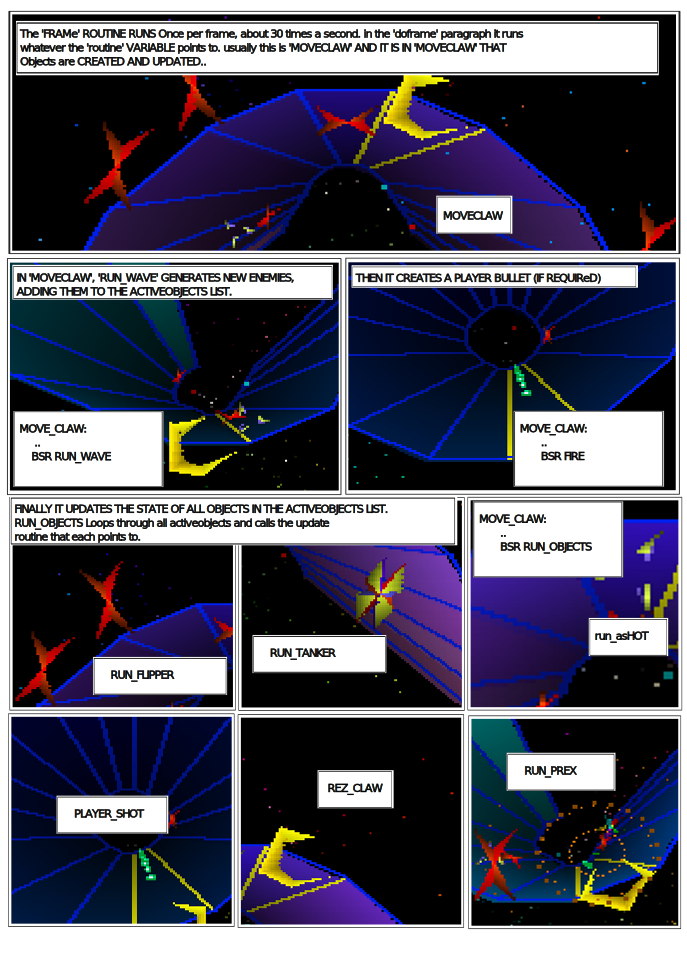
\includegraphics[width=13.7cm]{src/mainloop/mainloop-run_objects-comic.png}%
\end{figure}

\begin{lstlisting}
Frame:
        movem.l d0-d5/a0-a2,-(a7)   ; Stash values in d0-d5 and a0-a2
    
        ; Check if we're in a vertical blank or not.
fr:     move INT1,d0
        move d0,-(a7)              ; Stash some values in the stack so we can restore them later.
        btst #0,d0                 ; Are we in a vertical blank?
        beq CheckTimer             ; If not, skip everything and check for input only.
    
        ; We're in a vertical blank so can update some state.
        ; Copy the display list we built in 'blist' to 'dlist'. The
        ; display list will be used by the Objects Processor to paint
        ; the next frame. The pixel data for all the objects in the display
        ; list was generated by the most recent run of 'draw_objects' in
        ; 'mainloop'.
        movem.l d6-d7/a3-a6,-(a7)   ; Stash data and address registers.
        move.l blist,a0            ; Stash blist in a0.
        move.l dlist,a1            ; Stash dlist in a1.
        ; Copy all bytes in blist to dlist.
        move.l #$30,d0             ; 0x30 units of 4 bytes each to be copied.
xlst:   move.l (a0)+,(a1)+         ; Copy 4 bytes from blist to dlist.
        dbra d0,xlst               ; Keep copying until we run out of bytes.
    
        ; Build the display list for the next frame.
        bsr RunBeasties            ; build the next one
    
        ; Minter: "this code writes the proper screen address to double buffered objects in the display list."
        ; In 'main_loop' we prepare dscreen (double-buffered screen) with objects drawn by the GPU/Blitter. Once it's ready
        ; we set screen_ready. Here we check if screen_ready is set and if so, we swap dscreen into
        ; 'cscreen' (current screen). We will then update the main screen object in the Display List to
        ;  reference this new address.
        ; Check if we can swap in the new screen prepared in 'mainloop'.
setdb:  tst screen_ready           ; has 'mainloop' finished preparing a new screen?
        beq no_new_screen          ; If no, go to no_new_screen.
        tst sync                   ; Has mainloop signalled it safe to swap screens?
        beq no_new_screen          ; If no, go to new_screen.
    
        ; Swap dscreen into cscreen so that the new screen can be used in the Object List.
        move.l cscreen,d1          ; Stash cscreen in d1.
        move.l dscreen,cscreen     ; Overwrite cscreen with dscreen.
        move.l d1,dscreen          ; Overwrite dscreen with stashed cscreen.
        clr screen_ready           ; Signal that a new screen is required before we come here again.
        clr sync                   ; Signal to mainloop it can build a new screen.
    
        ; Check if we have a new screen to display.
no_new_screen:
        move.l dlist,a0            ; Point a0 at the display list.
        move db_on,d7              ; Is double-buffering enabled?
        bmi no_db                  ; If not, skip to warp flash.
    
        ; Update the main screen item in the Object List with the address of the new screen contained
        ; in cscreen. This has the effect of ensuring all the objects we drew with the GPU
        ; and Blitter in 'mainloop' are actually written to the screen by the Object Processor.
stdb:   move.l cscreen,d6          ; Get address of current displayed screen
        and.l #$fffffff8,d6        ; lose three LSB's
        lsl.l #8,d6                ; move to correct bit position
        move.l (a0),d1             ; get first word of the BMO
        and.l #$7ff,d1             ; clear data pointer
        or.l d6,d1                 ; mask in new pointer
        move.l d1,(a0)             ; replace in OL
        lea 32(a0),a0              ; This skips to the next object but is unnecessary since we are
                            ; only updating one item (the main screen) in the Object List with
                            ; our new screen pointer.
    
        ; Do the warp flash effect.
no_db:  jsr dowf                   ; Call the warp flash effect.
    
        ; Now do some magic for NTSC displays. If this is an NTSC display we want to skip playing
        ; sounds every 5th and 6th interrupt for some reason.
        tst pal                    ; Are we a PAL display?
        bne dtoon                  ; If no, we can skip this part.
        add #1,tuntime             ; Increment our visit count.
        cmp #4,tuntime             ; Less than 4?
        ble dtoon                  ; If less than 4, go ahead and play a sound.
        cmp #6,tuntime             ; Is it 6?
        bne ntoon                  ; If not, skip playing a sound this time.
        clr tuntime                ; If it is 6, reset to zero.
    
        ; Something to do with the Imagitec sound chip. Probably whether we should play
        ; a sound during the interrupt?
dtoon:  tst modstop                ; Is sound turned off?
        bne ntoon                  ; If yes, don't play a sound.
        jsr NT_VBL                 ; If no, play the next sound using the Imagitec sound synth.
    
        ; Do any in-game effects.
ntoon:  tst pawsed                 ; Are we paused?
        bne zial                   ; If so, skip.
        add #1,frames              ; Add to the number of frames.
        move.l fx,a0               ; Stash the current 'fx' routine in a0.
        jsr (a0)                   ; Run the routine.
    
        ; 'mainloop' might be busy processing stuff in the 'activeobjects' list. If it is,
        ; we will have to skip doing anything in this frame.
zial:   tst locked                 ; Are we in the middle of adding stuff to activeobjects?
        beq doframe                ; If not, do our context-specific per-frame routine.
        bra loseframe              ; If we're busy, skip this frame.
    
        ;
        ; Perform any context specific updates for this frame.
        ; 'routine' can be any one of:
        ;  - rrts, pauson, pausing, budb, pausoff, paws, zoom1, zoomto,
        ;    waitfor, zprev, znext, zshow, oselector, seldb, tunrun, text_o_run,
        ;    m7run, vicrun, failcount, viccount, txen, tgoto, rotate_web,
        ;    zoom3, zap_player, take_me_to_your_leader, snatch_it_away,
        ;    moveclaw, zoom2
        ;
        ; rotate_web -> moveclaw -> zoom1 -> zoom2 ->
        ; zoomto -> waitfor -> zprev -> zshow -> waitfor
        ;                   -> znext -> zshow
        ;                   -> rrts
        ; oselector ->seldb -> oselector
        ; _tunn -> tunrun ->
        ;
        ; The main update to the state of all objects is called from moveclaw.
        ; This calls run_objects which will update the state of everything in the
        ; activeobjects list.
doframe:
        move.l routine,a0          ; Stash the current 'routine' in a0.
        jsr (a0)                   ; Run it.
        clr drawhalt               ; This is redundant, it is never set anywhere.
    
loseframe:
        bsr checkpause             ; Check if the player has requested to pause the game.
        bsr domod                  ; Play a frame of music in the Imagitec synth.
        btst.b #0,sysflags         ; Check for hardware interlacing.
        bne chit                   ; If not enabled, skip.
    
        ; Some kind of fixing up for hardware interlace mode.
        move frames,d0             ; Stash frames in d0.
        and #$01,d0                ; Get the lsb.
        add #SIDE,d0               ; Add SIDE.
        sub palside,d0             ; Subtract PAL side.
        move d0,beasties           ; Store in beasties.
    
chit:   movem.l (a7)+,d6-d7/a3-a6   ; Restore values to data and address registers we stashed at the start.
    
CheckTimer:
        move (a7)+,d0              ; Restore stashed d0.
        move d0,-(a7)              ; Stash it again.
        btst #3,d0                 ; Do we need to check for joypad in put?
        beq exxit                  ; No, we can exit the interrupt.
    
        ; Check for joypad input. The logic for rotary controllers was added to support
        ; the potential release of a rotary controller for the Jaguar, but this never happened.
        ; So all rotary controller logic in Tempest 2000 is unused.
        tst roconon                ; Is Rotary Controller enabled?
        bne roco                   ; Yes, do the rotary controller.
        jsr dopad                  ; No, check for normal joypad in put.
        bra exxit                  ; We're done - so exit interrupt.
    
        ; Logic for reading input from the never-built and never-released rotary controller.
roco:   move pitcount,d1           ; Get the rotary input interval counter.
        and #$07,d1                ; Do a modulus 7 on the counter.
        bne rotonly                ; If non-zero, read the rotary control only.
        jsr dopad                  ; Otherwise, look for button presses too.
rotonly:
        add #1,pitcount            ; Increment the interval counter.
        bsr readrotary             ; Read input from the rotary controller.
    
        ; Minter: "Yeah, interrupts at 8x normal speed, go do special stuff."
exxit:
        move (a7)+,d0              ; Restore stashed d0.
        lsl #8,d0                  ; Shift left 8 bits.
        move.b intmask,d0          ; Add our interrupt mask.
        move d0,INT1               ; Add to INT1.
        move d0,INT2               ; Add to INT2.
        movem.l (a7)+,d0-d5/a0-a2   ; Restore stashed values.
        rte                        ; Return from the interrupt.
\end{lstlisting}
